\documentclass{SGGW-thesis}

\INZYNIERSKAtrue
\WZIMtrue

\title{Automatyczne rozpoznawanie\\instrumentów muzycznych\\w nagraniu audio}
\Etitle{Automatic Recognition of Musical Instruments\\in an Audio Recording}
\author{Grzegorz Marczewski}
\date{2025}
\album{210895}
\thesis{Praca dyplomowa na kierunku:}
\course{Informatyka}
\promotor{dra\ inż.\ Piotra Wrzeciono}
\pworkplace{Instytut Informatyki Technicznej\\Laboratorium Pomiarów Akustycznych}

\usepackage{listings}
\usepackage{xcolor}
\usepackage{amsmath}
\usepackage{graphicx}
\usepackage{multirow}
\usepackage{booktabs}
\usepackage{float}
\usepackage{hyperref}

\lstset{
  basicstyle=\ttfamily\small,
  keywordstyle=\color{blue},
  commentstyle=\color{gray},
  stringstyle=\color{red},
  numbers=left,
  numbers=none,
  frame=single,
  breaklines=true,
  showstringspaces=false,
  tabsize=2,
  language=Python
}


\begin{document}
\maketitle
\statementpage
\abstractpage
{Automatyczne rozpoznawanie instrumentów muzycznych w nagraniu audio}
{Celem pracy było porównanie skuteczności trzech metod w zadaniu rozpoznawania instrumentów muzycznych na podstawie cech dźwiękowych: SVM wykorzystującego statystyki MFCC, CNN wykorzystującego MFCC oraz CNN wykorzystującego mel-spektrogramy. Uczenie i testy przeprowadzono na zbiorach Kaggle (16 klas, pojedyncze instrumenty) oraz IRMAS (11 klas, instrumenty dominujące). Najlepsze wyniki uzyskano przy użyciu CNN z mel-spektrogramami: dokładność 92\% dla Kaggle oraz 75\% dla IRMAS. Model CNN z MFCC osiągnął odpowiednio 92\% i 69\%, a SVM 78\% i 48\%. Wyniki potwierdzają wyższą skuteczność głębokich sieci, a dla bardziej złożonych danych przewagę wykorzystania mel-spektrogramów w porównaniu do MFCC w przypadku CNN.}
{TensorFlow, SVM, CNN, MFCC, mel-spektrogram}
{Automatic Recognition of Musical Instruments in an Audio Recording}
{The aim of this study was to compare the effectiveness of three methods in the task of musical instrument recognition based on audio features: SVM classifier using MFCC statistics, CNN using MFCC and CNN using mel-spectrograms. Training and tests were performed on the Kaggle dataset (16 classes, single instruments) and the IRMAS dataset (11 classes, dominant instruments). The best results were achieved using CNN with mel-spectrograms: 92\% accuracy for Kaggle and 75\% for IRMAS. The CNN model with MFCC achieved 92\% and 69\%, respectively, while the SVM model achieved 78\% and 48\%. The results confirm the higher effectiveness of deep networks, and for more complex data, the advantage of using mel-spectrograms over MFCC in the case of CNN.}
{TensorFlow, SVM, CNN, MFCC, mel-spectrogram}




\tableofcontents

\startchapterfromoddpage




\chapter{Wstęp}

Rozpoznawanie instrumentów muzycznych na podstawie nagrań audio stanowi jedno z głównych wyzwań w dziedzinie przetwarzania dźwięku. W ostatnich latach, dzięki postępom w uczeniu maszynowym, w szczególności w zakresie głębokich sieci neuronowych, osiągnięto znaczące postępy w zadaniach związanych z automatycznym klasyfikowaniem instrumentów muzycznych. Tradycyjne metody klasyfikacji, takie jak maszyny wektorów nośnych (SVM), wciąż stanowią solidną alternatywę, szczególnie w przypadkach, gdy zasoby obliczeniowe są ograniczone. Z kolei konwolucyjne sieci neuronowe (CNN) zyskały na popularności dzięki swojej zdolności do wykrywania skomplikowanych wzorców w danych, takich jak obrazy, dźwięki czy inne formy sygnałów. Do reprezentacji cech audio w analizie dźwięku często wykorzystuje się współczynniki MFCC oraz mel-spektrogramy, które umożliwiają uchwycenie istotnych informacji o charakterystyce dźwięku, ułatwiając rozpoznawanie instrumentów muzycznych.

\section{Cel i zakres pracy}
Celem niniejszej pracy jest porównanie skuteczności trzech metod uczenia maszynowego w zadaniu rozpoznawania instrumentów muzycznych na podstawie cech dźwiękowych. Praca skupia się na klasyfikatorze SVM wykorzystującym statystyki MFCC oraz dwóch wariantach konwolucyjnej sieci neuronowej (CNN): jednym, który stosuje współczynniki MFCC, oraz drugim, który wykorzystuje mel-spektrogramy. Celem jest analiza efektywności tych trzech podejść w kontekście różnych reprezentacji danych audio. Eksperymenty przeprowadzono na dwóch zbiorach danych: IRMAS, zawierającym nagrania z dominującym instrumentem, oraz Kaggle, zawierającym nagrania pojedynczych instrumentów.




\chapter{Przegląd literatury}

\section{Podstawy teoretyczne}

\subsection{Machine Learning}
\textbf{Uczenie maszynowe} (Machine Learning) to dziedzina sztucznej inteligencji, której celem jest tworzenie algorytmów umożliwiających komputerom automatyczne doskonalenie swojej wydajności w wykonywaniu określonych zadań na podstawie doświadczenia, czyli danych treningowych. Uczenie maszynowe dzieli się na nadzorowane (supervised), nienadzorowane (unsupervised) oraz wzmacniające (reinforcement learning)~\cite{mitchell1997machine}.

\subsection{SVM}
\textbf{Maszyna wektorów nośnych} (Support Vector Machine, SVM) to algorytm nadzorowanego uczenia maszynowego wykorzystywany do klasyfikacji oraz regresji. Celem SVM jest znalezienie hiperpłaszczyzny (w przestrzeni cech), która najlepiej oddziela dane należące do różnych klas, maksymalizując margines. W przypadku danych nieliniowo separowalnych SVM używa funkcji jądra (kernel), aby przekształcić dane do przestrzeni o wyższej wymiarowości, gdzie możliwe jest znalezienie liniowej granicy decyzyjnej~\cite{moguerza2006support}. 

\subsection{Neural network}
\textbf{Sieci neuronowe} (Neural Networks) to modele obliczeniowe inspirowane ludzkim mózgiem, składające się z neuronów ułożonych w warstwy. Neurony w sieci przetwarzają dane, przekazując wyniki do kolejnych warstw. Sieć zawiera warstwę wejściową, ukrytą i wyjściową. Proces uczenia polega na modyfikacji wag połączeń między neuronami na podstawie błędów prognozy, zwykle przy użyciu algorytmu backpropagation~\cite{goodfellow2016deep}.

\subsection{Deep learning}
\textbf{Głębokie uczenie} (Deep Learning) to poddziedzina uczenia maszynowego, w której wykorzystywane są sieci neuronowe o wielu warstwach ukrytych. Dzięki tej głębi możliwe jest sprowadzenie skomplikowanych konceptów do relacji pomiędzy prostymi zależnościami. Deep Learning najduje zastosowanie w rozpoznawaniu obrazów, mowy czy dźwięku~\cite{goodfellow2016deep}.

\subsection{CNN}
\textbf{Konwolucyjna sieć neuronowa} (Convolutional Neural Network, CNN) to specjalna architektura sieci neuronowej wykorzystywana głównie do analizy danych obrazowych. CNN składają się z warstw konwolucyjnych, poolingowych i gęsto połączonych. Dzięki warstwom konwolucyjnym sieci te są w stanie wykrywać złożone wzorce w danych wejściowych~\cite{goodfellow2016deep}.

\subsection{Spektrogram}
\textbf{Spektrogram} to trójwymiarowa reprezentacja sygnału dźwiękowego, w której dwie osie odpowiadają czasowi i częstotliwości, natomiast trzecia zmienna, czyli amplituda lub energia, odwzorowywana jest za pomocą koloru lub intensywności punktu. Alternatywnie, spektrogram może być przedstawiany jako trójwymiarowa powierzchnia, gdzie amplituda stanowi oś pionową (z), co umożliwia przestrzenną wizualizację zmian widma w czasie. Spektrogram otrzymuje się poprzez podział sygnału na krótkie, nakładające się na siebie ramki, dla których obliczana jest szybka transformata Fouriera (FFT). Ramki te wyznaczane są z użyciem funkcji okna czasowego, która ogranicza fragment sygnału w dziedzinie czasu i redukuje efekt przecieków widmowych~\cite{smith1997scientist}.

FFT sygnału $x[n]$ jest zdefiniowana w równaniu~\eqref{eq:fft}:
\begin{equation}
X[k] = \sum_{n=0}^{N-1} x[n] e^{-j \frac{2\pi}{N}kn}
\label{eq:fft}
\end{equation}

gdzie:
\begin{itemize}
    \renewcommand{\labelitemi}{}
    \item $x[n]$ – próbki analizowanego sygnału dyskretnego,
    \item $N$ – liczba próbek (długość sygnału),
    \item $k$ – indeks częstotliwości, $k = 0, 1, \dots, N - 1$,
    \item $j$ – jednostka urojona, dla której $j^2 = -1$.
\end{itemize}

Przykładowe okna czasowe wykorzystywane w STFT do segmentacji sygnału są zdefiniowane w równaniach~\ref{eq:hann}, \ref{eq:hamming}, \ref{eq:blackman}, \ref{eq:flattop}, \ref{eq:bartlett}:
\begin{itemize}
    \item \textbf{Okno Hanninga (Hann window)}:
    \begin{equation}
    w[n] = 0{,}5 \left( 1 - \cos\left(\frac{2\pi n}{N - 1}\right) \right)
    \label{eq:hann}
    \end{equation}
    \item \textbf{Okno Hamminga (Hamming window)}:
    \begin{equation}
    w[n] = 0{,}53836 - 0{,}46164 \cos\left(\frac{2\pi n}{N - 1}\right)
    \label{eq:hamming}
    \end{equation}
    \item \textbf{Okno Blackmana (Blackman window)}:
    \begin{equation}
    w[n] = a_0 - a_1 \cos\left(\frac{2\pi n}{N - 1}\right) + a_2 \cos\left(\frac{4\pi n}{N - 1}\right)
    \label{eq:blackman}
    \end{equation}
    gdzie: \\
    $a_0 = 0{,}42$; $a_1 = 0{,}5$; $a_2 = 0{,}08$
    \item \textbf{Okno Flat top (Flat top window)}:
    \begin{equation}
    w[n] = a_0 - a_1 \cos\left(\frac{2\pi n}{N - 1}\right) + a_2 \cos\left(\frac{4\pi n}{N - 1}\right) - a_3 \cos\left(\frac{6\pi n}{N - 1}\right) + a_4 \cos\left(\frac{8\pi n}{N - 1}\right)
    \label{eq:flattop}
    \end{equation}
    gdzie: \\
    $a_0 = 1$; $a_1 = 1{,}93$; $a_2 = 1{,}29$; $a_3 = 0{,}388$; $a_4 = 0{,}028$
    \item \textbf{Okno Bartlett (Bartlett window)}:
    \begin{equation}
    w[n] = 1 - \left| \frac{n - \frac{N-1}{2}}{\frac{N-1}{2}} \right|
    \label{eq:bartlett}
    \end{equation}
\end{itemize}

\subsection{Zasada nieoznaczoności Heisenberga}

Zasada nieoznaczoności Heisenberga, znana głównie z mechaniki kwantowej, znajduje również zastosowanie w analizie sygnałów, w szczególności w kontekście transformaty Fouriera. Zasada ta odnosi się do fundamentalnego ograniczenia w jednoczesnym określaniu precyzyjnej lokalizacji sygnału zarówno w dziedzinie czasu, jak i częstotliwości. Im krótszy (bardziej zlokalizowany w czasie) jest analizowany sygnał, tym szersze jest jego widmo częstotliwościowe, i odwrotnie, sygnał dobrze zlokalizowany w częstotliwości musi być rozciągnięty w czasie. Oznacza to, że nie da się jednocześnie uzyskać wysokiej rozdzielczości czasowej i częstotliwościowej. 

W praktyce wpływ tej zasady widoczny jest w spektrogramach, które uzyskuje się poprzez podział sygnału na nakładające się segmenty czasowe przy pomocy funkcji okna, a następnie obliczenie szybkiej transformaty Fouriera (FFT) dla każdego segmentu. Wybór długości okna wpływa na kompromis pomiędzy rozdzielczością czasową a częstotliwościową: krótkie okna lepiej odwzorowują zmiany w czasie, natomiast długie, zmiany częstotliwościowe~\cite{bracewell2000fourier}.

\subsection{Prawo Webera-Fechnera}

Prawo Webera-Fechnera jest kluczowym konceptem w psychofizyce, które opisuje, jak ludzkie zmysły postrzegają zmiany w intensywności bodźców. Zgodnie z tym prawem, percepcja różnicy między dwoma bodźcami jest proporcjonalna do logarytmicznego stosunku zmiany intensywności bodźca do jego początkowej wartości. Dla niższych wartości intensywności zmiany są łatwiejsze do zauważenia, podczas gdy w wyższych wartościach nasza zdolność do rozróżniania różnic jest znacznie mniej precyzyjna. Matematyczną definicję prawa Fechnera opisano w równaniu \ref{eq:weber_fechner}.

\begin{equation}
    \Delta S = k \log\left(\frac{I_2}{I_1}\right)
    \label{eq:weber_fechner}
\end{equation}

gdzie:
\begin{itemize}
    \renewcommand{\labelitemi}{}
    \item \( \Delta S \) – zmiana percepcji wrażenia (np. głośności),
    \item \( I_2 \) – końcowa intensywność bodźca,
    \item \( I_1 \) – początkowa intensywność bodźca,
    \item \( k \) – stała Fechnera, która zależy od rodzaju bodźca (np. dźwięk, światło).
\end{itemize}

Wzór ten mówi, że różnica w percepcji \( \Delta S \) jest proporcjonalna do logarytmu stosunku intensywności bodźców \( I_2 \) i \( I_1 \). Stała \( k \) jest wyznaczana eksperymentalnie i różni się w zależności od rodzaju bodźca.

Choć prawo Fechnera dobrze odwzorowuje percepcję zmiany intensywności w średnich zakresach, ma swoje ograniczenia, szczególnie przy bardzo niskich lub bardzo wysokich poziomach intensywności. Przy bardzo niskich intensywnościach percepcja zmiany nie jest liniowa, a dla bardzo wysokich poziomów intensywności zdolność rozróżniania zmian także maleje. Ponadto, prawo Fechnera nie uwzględnia w pełni kontekstu psychofizycznych różnic indywidualnych, takich jak próg percepcji czy wpływ zmiennych zewnętrznych~\cite{gescheider2013psychophysics}.


\subsection{Skala melowa}

Skala melowa to nieliniowa skala częstotliwości, zaprojektowana w taki sposób, aby lepiej odwzorować sposób, w jaki ludzkie ucho postrzega różne częstotliwości, wykorzystując wiedzę z prawa Webera-Fechnera. Nazwa skali melowej pochodzi od słowa „melodia”, ponieważ skala ta została nieświadomie wykorzystywana w muzyce w kontekście tworzenia melodii. W rzeczywistości, w tradycyjnej muzyce, interwały między dźwiękami były dobierane w sposób, który odpowiadał subiektywnej percepcji ludzkiego słuchu, zwłaszcza w zakresie częstotliwości, w którym ucho jest najbardziej wrażliwe.

Transformacja z częstotliwości liniowej na melową jest opisana w równaniu \ref{eq:mel}:

\begin{equation}
\text{Mel}(f) = 2595 \cdot \log_{10} \left( 1 + \frac{f}{700} \right)
\label{eq:mel}
\end{equation}

gdzie:
\begin{itemize}
    \renewcommand{\labelitemi}{}
    \item \( f \) – częstotliwość w Hz,
    \item \( \text{Mel}(f) \) – częstotliwość wyrażona w jednostkach meli.
\end{itemize}


\subsection{MFCC}
\textbf{Współczynniki Mel-Cepstralne} (Mel Frequency Cepstral Coefficients, MFCC) to reprezentacja cech dźwięku, powszechnie stosowana w rozpoznawaniu mowy i dźwięków. MFCC opierają się na ludzkim postrzeganiu częstotliwości (skala melowa). Współczynniki te są uzyskiwane poprzez poddanie sygnału audio transformacji cepstralnej. Dolne współczynniki odpowiadają za barwę dźwięku (timbre) instrumentów, podczas gdy górne współczynniki mogą zawierać informacje o ataku dźwięku i harmonii. Dzięki tym cechom MFCC są bardzo pomocne w klasyfikacji instrumentów muzycznych, ponieważ pozwalają rozróżnić instrumenty na podstawie ich unikalnych cech akustycznych~\cite{jadhav2015classification}.

Pierwszym krokiem w transformacji cepstralnej jest obliczenie spektrogramu sygnału, który przedstawia rozkład energii w czasie i częstotliwości. Następnie, spektrogram jest przekształcany na skalę melową, której częstotliwości odpowiadają postrzeganemu przez człowieka rozkładowi częstotliwości. Kolejnym krokiem jest logarytmowanie amplitudy każdej próbki w tym spektrogramie. Na końcu stosuje się dyskretną transformację kosinusową (DCT).

Dyskretna transformacja kosinusowa (DCT) przedstawiona jest w równaniu~\ref{eq:dct}:
\begin{equation}
X_k = \sum_{n=0}^{N-1} x_n \cos \left[ \frac{\pi}{N} \left( n + \frac{1}{2} \right) k \right], \quad k = 0, 1, 2, \dots, N-1
\label{eq:dct}
\end{equation}

gdzie:
\begin{itemize}
    \renewcommand{\labelitemi}{}
    \item \( X_k \) – współczynniki DCT (transformacji kosinusowej),
    \item \( x_n \) – logarytmowane amplitudy widma na skali melowej dla \( n \)-tej częstotliwości,
    \item \( N \) – liczba współczynników DCT,
    \item \( k \) – indeks współczynnika DCT,
    \item \( n \) – indeks próbki w skali melowej.
\end{itemize}

Transformacja ta pozwala uzyskać skompaktowaną reprezentację sygnału, eliminując zmienność wynikającą z intensywności i fazy, co jest kluczowe dla dalszej analizy akustycznej i klasyfikacji dźwięków.

\subsection{Mel-spektrogram}
\textbf{Mel-spektrogram} to spektrogram, w którym oś częstotliwości jest przekształcona zgodnie ze skalą melową, odzwierciedlającą sposób postrzegania dźwięków przez ludzkie ucho. Proces tworzenia mel-spektrogramu polega na obliczeniu klasycznego spektrogramu, a następnie zastosowaniu banku filtrów melowych, który agreguje energie wzdłuż osi częstotliwości w skali melowej. Mel-spektrogram stanowi trójwymiarową macierz (czas $\times$ mel-częstotliwość $\times$ amplituda), co sprawia, że może być traktowany i analizowany jak obraz. Dzięki swoim właściwościom perceptualnym, mel-spektrogram jest szeroko stosowany jako wejście do modeli uczenia maszynowego, szczególnie w zadaniach rozpoznawania mowy i dźwięku~\cite{thornton2019audio}.

\section{Przegląd dotychczasowych badań}
Eronen (2001)~\cite{eronen2001automatic} przeprowadził analizę skuteczności różnych cech akustycznych, takich jak współczynniki MFCC, cechy spektrogramowe oraz cechy związane z barwą dźwięku, w kontekście rozpoznawania instrumentów muzycznych. Zastosowane klasyczne algorytmy uczenia maszynowego, takie jak k-NN (k-Nearest Neighbors), pozwoliły na zbadanie wpływu reprezentacji czasowej i częstotliwościowej na jakość klasyfikacji. Wyniki pokazały, że odpowiedni dobór cech jest kluczowy dla skuteczności rozpoznawania instrumentów, co potwierdza znaczenie wyboru odpowiednich reprezentacji akustycznych w tego typu zadaniach.

Herrera-Boyer, Peeters i Dubnov (2003)~\cite{herrera2003automatic} dokonali przeglądu metod automatycznej klasyfikacji dźwięków instrumentów muzycznych, zwracając szczególną uwagę na cechy opisujące barwę dźwięku. Podkreślili znaczenie współczynników MFCC, które wykazują wysoką efektywność zarówno w zadaniach rozpoznawania mowy, jak i instrumentów muzycznych. Mimo swoich ograniczeń, takich jak brak informacji o dynamice czasowej, MFCC pozostają jedną z najefektywniejszych cech statycznych w rozpoznawaniu instrumentów.

Wieczorkowska i Czyżewski (2003)~\cite{wieczorkowska2003rough} zaprezentowali zastosowanie teorii zbiorów przybliżonych do klasyfikacji dźwięków instrumentów muzycznych. Podejście to pozwoliło na uzyskanie wysoce precyzyjnych wyników, zwłaszcza w przypadku dźwięków o złożonej strukturze harmonicznej, co stanowiło istotne wyzwanie w kontekście rozpoznawania instrumentów. Autorka wykorzystała cechy wyekstraktowane z transformaty Fouriera oraz analizy falkowej, co umożliwiło dokładniejszą identyfikację barwy dźwięku.

Wieczorkowska i Kolczyńska (2008)~\cite{wieczorkowska2008identification} zaproponowały nowe podejście do rozpoznawania dominujących instrumentów w nagraniach, które zawierały instrumenty o tej samej wysokości dźwięku. Skupiły się na wykorzystaniu klasyfikatorów SVM z nieliniowym jądrem do rozpoznawania dominującego instrumentu w polifonicznych miksach dźwięków o identycznej wysokości. Badania obejmowały analizę dźwięków z jednej oktawy dwunastu instrumentów, zarówno w formie izolowanej, jak i w mieszankach z dodanymi sztucznymi dźwiękami harmonicznymi i szumami o niższej amplitudzie.

Jiang, Wieczorkowska i Raś (2009)~\cite{jiang2009music} zaprezentowali metodę klasyfikacji instrumentów muzycznych w nagraniach polifonicznych, opartą na dopasowaniu krótkoterminowego widma dźwięku. Dzięki tej technice, przy użyciu m.in. algorytmu k-NN, udało się skutecznie rozróżniać instrumenty w złożonych nagraniach, w których dźwięki wielu instrumentów nakładają się na siebie.

Bosch, Janer, Fuhrmann i Herrera (2012)~\cite{bosch2012comparison} zaprezentowali zbiór danych IRMAS (Instrument Recognition in Musical Audio Signals), który zawiera nagrania muzyczne z rzeczywistych utworów. Zbiór ten stał się powszechnie używanym narzędziem w badaniach nad automatycznym rozpoznawaniem instrumentów muzycznych, ponieważ zawiera różnorodne utwory, które lepiej odwzorowują warunki rzeczywiste w porównaniu do syntetycznych danych. W pracy zastosowano klasyfikator SVM oraz MFCC, a wyniki pokazały, że dobór odpowiednich cech w połączeniu z klasyfikatorami SVM może prowadzić do wysokiej skuteczności w rozpoznawaniu instrumentów w nagraniach muzycznych.

Badanie autorstwa Kubera, Wieczorkowskiej i Rasia (2013)~\cite{kubera2013time} zaprezentowało hierarchiczne podejście do rozpoznawania instrumentów muzycznych, oparte na analizie zmienności czasowej sygnału. Dzięki tej metodzie udało się skutecznie klasyfikować instrumenty, a także identyfikować więcej niż jeden instrument w nagraniu, co miało zastosowanie w nagraniach polifonicznych. Dodatkowo, eksperymenty wykazały, że ta technika przynosi lepsze wyniki w porównaniu do tradycyjnych klasyfikatorów płaskich, które bezpośrednio szacują instrumenty, oraz klasyfikatorów opartych na klasycznym schemacie Hornbostela-Sachsa.

Kursa i Wieczorkowska (2014)~\cite{kursa2014multi} przedstawili nowatorskie podejście oparte na algorytmach typu multi-label Ferns, które pozwalały na efektywne rozpoznawanie instrumentów muzycznych w nagraniach. Skupili się na opracowaniu algorytmu, który mógłby poradzić sobie z klasyfikacją wielu instrumentów w jednym nagraniu audio, uwzględniając specyficzne cechy dźwięków z różnych rodzin instrumentów. Wyniki wykazały, że metoda ta może znacznie poprawić efektywność klasyfikacji w porównaniu do tradycyjnych podejść.

W pracy Solankiego i Pandeya (2022)~\cite{solanki2022music} zaproponowano zastosowanie głębokich konwolucyjnych sieci neuronowych (CNN) do zadania rozpoznawania instrumentów muzycznych. Autorzy zastosowali mel-spektrogramy jako dane wejściowe, które lepiej uwzględniają zarówno informację czasową, jak i częstotliwościową. Wykazano, że sieci CNN są bardzo skuteczne w ekstrakcji cech czasowo-częstotliwościowych, co czyni je odpowiednimi do takich zadań jak rozpoznawanie instrumentów. Ich badania wykazały, że odpowiedni dobór architektury sieci oraz parametrów treningowych pozwala na osiągnięcie wysokiej dokładności klasyfikacji, co jest istotnym osiągnięciem w dziedzinie rozpoznawania instrumentów na podstawie nagrań audio. Zastosowany model CNN składał się z czterech warstw konwolucyjnych i warstw poolingowych, osiągając dokładność klasyfikacji przekraczającą 90\% na zbiorze IRMAS, który obejmuje 11 instrumentów muzycznych.




\chapter{Opis zbiorów danych}

\section{ Zbiór Kaggle}
Pierwszym zbiorem danych, jaki wykorzystono w tej pracy, jest udostępniony na platformie Kaggle~\cite{howard2018freesound} zestaw nagrań zawierający, oprócz innych dźwięków, 1847 nieskompresowanych 16-bitowych plików mono PCM o częstotliwości próbkowania 44,1 kHz. Pliki te zostały ręcznie zaklasyfikowane i przedstawiają jeden z 16 instrumentów oznaczonych w bazie jako: hi-hat (Hi-hat), saksofon (Saxophone), trąbka (Trumpet), dzwonki (Glockenspiel), wiolonczela (Cello), klarnet (Clarinet), obój (Oboe), flet (Flute), bęben basowy (Bass drum), kontrabas (Double bass), tamburyn (Tambourine), krowi dzwonek (Cowbell), fortepian elektryczny (Electric piano), harmonijka ustna (Harmonica), gitara akustyczna (Acoustic guitar) oraz skrzypce (Violin or fiddle). Pliki te cechują się jednolitą jakością i przedstawiają brzmienie pojedynczych nut, skal dźwiękowych lub krótkich fraz melodycznych.

\section{ Zbiór IRMAS}
Drugi zbiór danych pochodzi ze strony IRMAS~\cite{bosch2012irmas} i zawiera 6705 plików audio w formacie WAV stereo 16-bitowym, próbkowanych w 44,1 kHz. Są to trzysekundowe wycinki utworów muzycznych, zawierających dominujący instrument, którego identyfikacja została dokonana manualnie. Instrumenty zaklasyfikowano jako jeden z 11 rodzajów oznaczonych w bazie: wiolonczela (cel), klarnet (cla), flet (flu), gitara akustyczna (gac), gitara elektryczna (gel), organy (org), fortepian (pia), saksofon (sax), trąbka (tru), skrzypce (vio) lub ludzki głos (voi), który w kontekście tej analizy traktowany jest jako instrument muzyczny. Oprócz głównego źródła dźwięku, w nagraniach występują także inne instrumenty. Zbiór ten cechuje różnorodność gatunkowa oraz jakościowa, przez co lepiej odzwierciedla naturalne występowanie instrumentów.

\section{Przygotowanie danych}
W poniższej sekcji przetwarzanie dźwięku zrealizowano z użyciem biblioteki librosa \cite{mcfee2015librosa}, a w operacjach na danych zastosowano biblioteki NumPy \cite{harris2020array} oraz pandas \cite{mckinney2010data}. 

Na początku, podczas ładowania plików dźwiękowych do przetwarzania, dokonano zmiany częstotliwości próbkowania z 44,1 kHz na 22,05 kHz. Zastosowano to rozwiązanie, ponieważ utracone częstotliwości mają znikomy wpływ na klasyfikację instrumentów muzycznych, a mniejszy rozmiar plików przyspiesza trenowanie modelu. W przypadku nagrań z bazy IRMAS dodatkowo przekonwertowano je ze stereo na mono, aby uprościć dane.

Następnie, dla modeli CNN, przeprowadzono segmentację nagrań na fragmenty o długości nieprzekraczającej jednej sekundy. W przypadku segmentów krótszych niż jedna sekunda ich długość została uzupełniona ciszą. Listing~\ref{lst:segmentation} przedstawia kod opisywanego działania.
\begin{lstlisting}[caption=Funkcja segmentująca nagranie na jednosekundowe fragmenty, label={lst:segmentation}, captionpos=b]
def segment_signal(y, delta_time=1, sr=22050):
    segment_length = int(delta_time * sr)
    segments = [y[i:i + segment_length] for i in range(0, len(y), segment_length)]
    
    fixed_segments = []
    for segment in segments:
        if len(segment) < segment_length:
            fixed_segments.append(np.pad(segment, (0, segment_length - len(segment)), mode='constant', constant_values=0))
        else:
            fixed_segments.append(segment)

    return fixed_segments
\end{lstlisting}

W kolejnym kroku nagrania zostały poddane normalizacji oraz usunięciu cichych fragmentów, co miało na celu polepszenie analizy dźwięku. Zastosowano obwiednię z oknem o długości 1/20 sekundy, która maskuje fragmenty, w których głośność nie przekracza 10\% maksymalnej amplitudy danego nagrania. Wybrano takie parametry, ponieważ dawały one najlepsze wyniki w eksperymentach. Działanie funkcji obwiedni przedstawiono w Listing~\ref{lst:envelope}, a wynik tej operacji pokazano na rysunku~\ref{fig:kaggle_envelope}.

\begin{lstlisting}[caption=Funkcja obwiedni do maskowania cichych fragmentów nagrań audio, label={lst:envelope}, captionpos=b]
def envelope(y, threshold=0.1, sr=22050):
    mask = []
    y = pd.Series(y).apply(np.abs)
    y_mean = y.rolling(window=int(sr/20),
                       min_periods=1,
                       center=True).max()
    
    for mean in y_mean:
        if mean > threshold:
            mask.append(True)
        else:
            mask.append(False)

    return mask, y_mean
\end{lstlisting}

\begin{figure}[H]
\centering
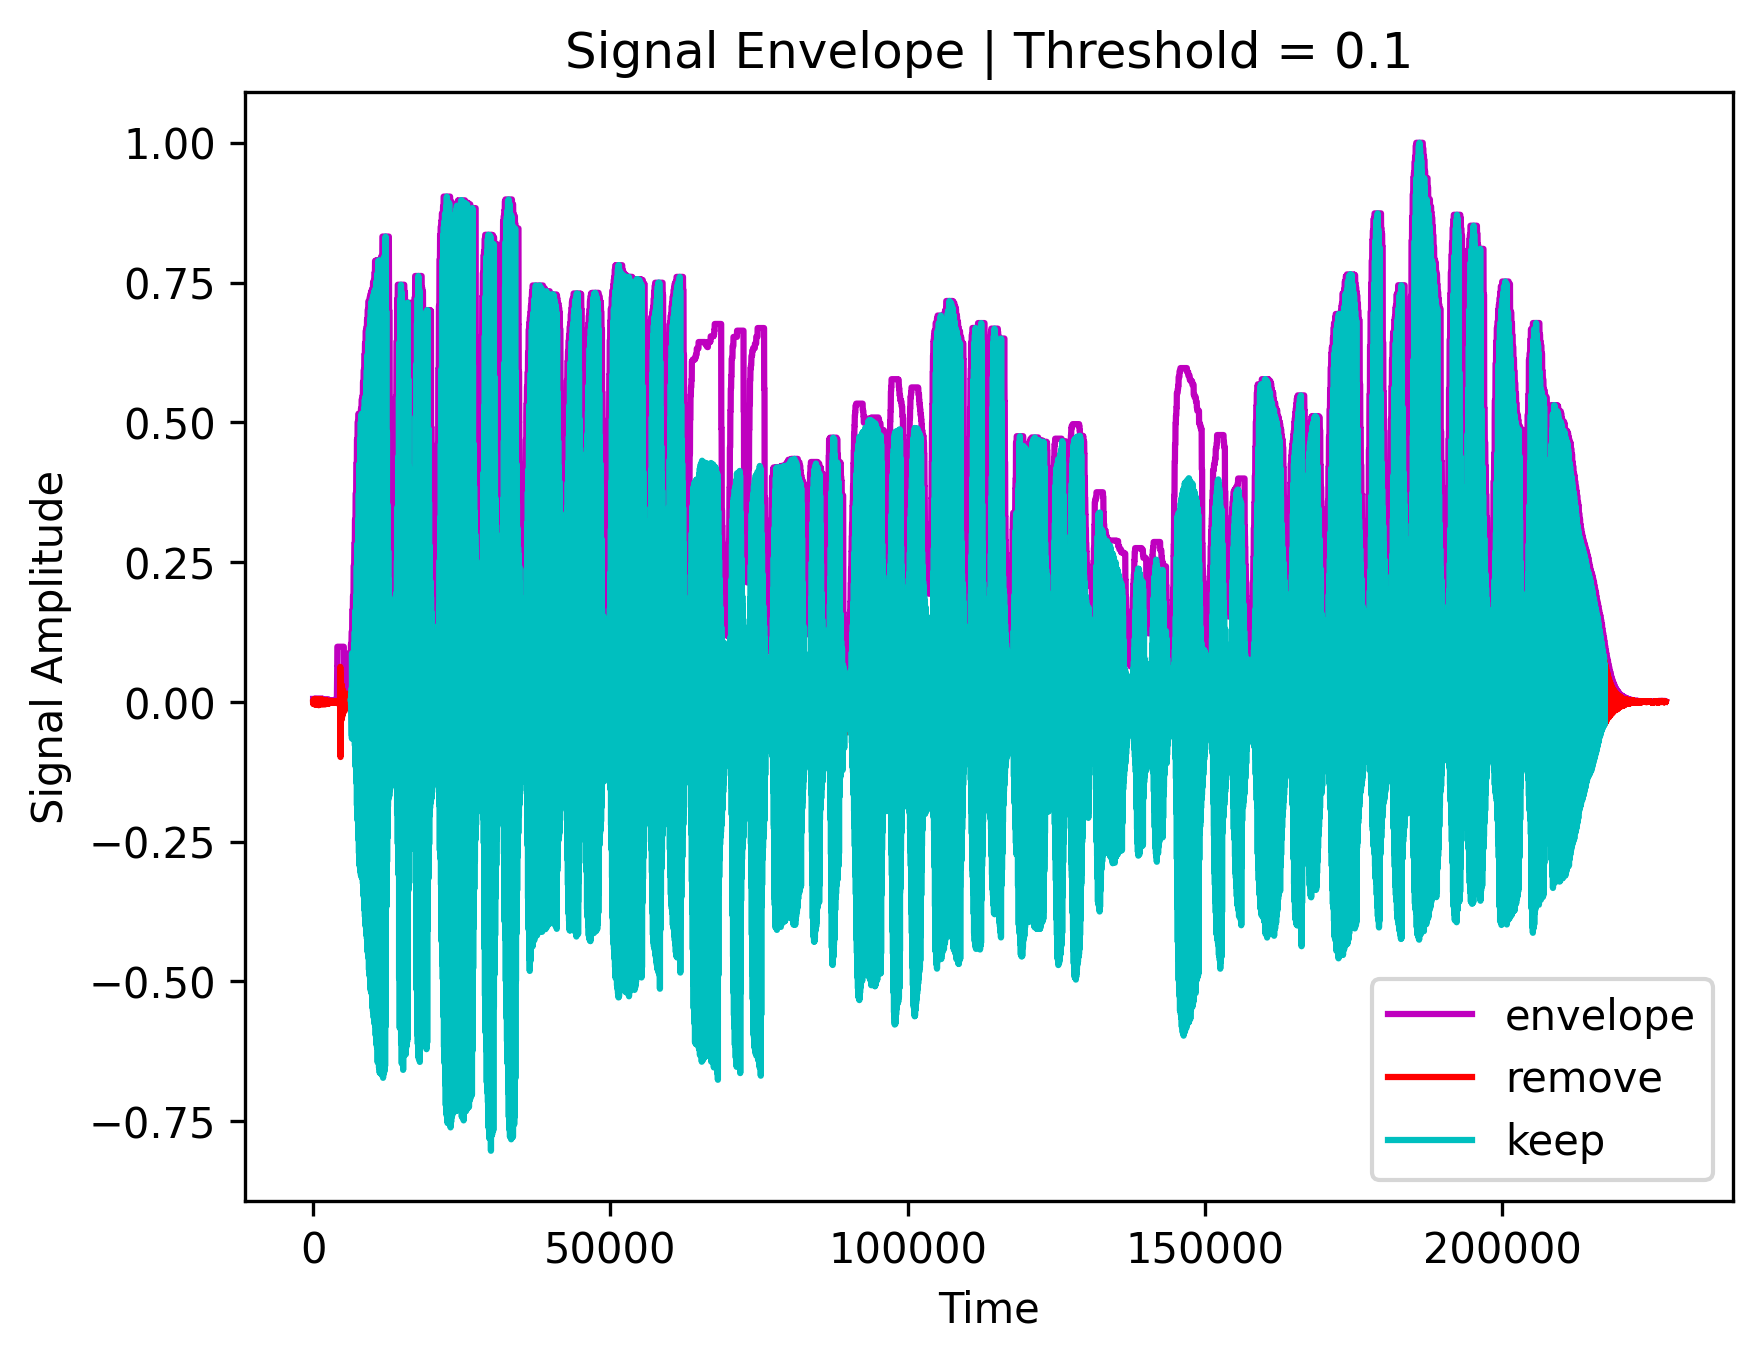
\includegraphics[width=0.8\textwidth]{kaggle_envelope.png}
\caption{Prezentacja działania funkcji maskującej ciche fragmenty na przykładzie nagrania z bazy Kaggle}
\label{fig:kaggle_envelope}
\end{figure}

\section{Podział zbiorów treningowych i testowych}
Dla każdego zbioru danych używanego w modelach CNN zastosowano podział z zachowaniem proporcji klas, wyodrębniając trzy zbiory:
\begin{itemize} 
    \item \textit{Train} -- próbki dźwiękowe używane do uczenia modelu, stanowiące 64\% danych. 
    \item \textit{Validation} -- zbiór walidacyjny obejmujący 16\% całości, służący do dostrajania hiperparametrów oraz oceny modelu w trakcie treningu. 
    \item \textit{Test} -- dane testowe stanowiące 20\% całości, wykorzystywane wyłącznie do ostatecznej oceny skuteczności modelu.
 \end{itemize}

W przypadku modeli SVM nastąpił podobny podział, jednak zbiór \textit{Validation} pozostał w zbiorze \textit{Train}, ponieważ dla tego typu modeli nie przeprowadza się walidacji z wykorzystaniem oddzielnego zbioru. Do podziału danych wykorzystano funkcję \textit{train\_test\_split} z biblioteki scikit-learn~\cite{pedregosa2011scikit}, z zastosowaniem parametru \textit{stratify} w celu zachowania proporcji klas. Dane ze zbioru Kaggle musiały zostać wstępnie przefiltrowane, aby odrzucić nagrania niedotyczące instrumentów muzycznych oraz te, które nie zostały oznaczone flagą wskazującą na manualną klasyfikację.




\chapter{Metody ekstrakcji cech}
\section{Wyliczenia średniej i odchylenia standardowego MFCC}
Dla modeli SVM, które cechują się niższą skutecznością w rozpoznawaniu skomplikowanych wzorców, wykorzystano wyłącznie statystyki MFCC. W tym celu obliczono współczynniki MFCC z oczyszczonych nagrań, a następnie dla każdego współczynnika zapisano jego średnią oraz odchylenie standardowe. Opisane działania przedstawiono w Listing~\ref{lst:mfcc_features}.

\begin{lstlisting}[caption=Funkcja obliczająca statystyki MFCC poszczególnych nagrań, label={lst:mfcc_features}, captionpos=b]
def create_mfcc_features(df, clean_dir, n_mfcc=13, hop_length=512):
    clean_dir = Path(clean_dir)
    mfcc_features_list = []
    
    for f in tqdm(df.fname):
        y, sr = librosa.load(clean_dir / f, sr=None)
        n_fft = min(2048, len(y))
        mfcc = librosa.feature.mfcc(y=y, 
                                    sr=sr, 
                                    n_mfcc=n_mfcc, 
                                    n_fft=n_fft, 
                                    hop_length=hop_length)
        mfcc_mean = np.mean(mfcc, axis=1)
        mfcc_std = np.std(mfcc, axis=1)
        mfcc_features = np.concatenate([mfcc_mean, mfcc_std])
        mfcc_features_list.append(mfcc_features)

    X = np.array(mfcc_features_list)
    y = df['label'].values

    return X, y
\end{lstlisting}

\section{Generowanie współczynników MFCC}
W przypadku pierwszych modeli CNN, z jednosekundowych segmentów utworzono MFCC składające się z 13 współczynników, przy zastosowaniu kroku wynoszącego 512 próbek. Kod tworzący MFCC przedstawiono w Listing~\ref{lst:mfcc}, a współczynniki MFCC zaprezentowano na rysunku~\ref{fig:kaggle_mfcc}.

\begin{lstlisting}[caption=Funkcja tworząca MFCC z jednosekundowego segmentu nagrania, label={lst:mfcc}, captionpos=b]
def create_mfcc(df, segmented_dir, all_categories, n_mfcc=13, hop_length=512):
    segmented_dir = Path(segmented_dir)
    mfcc_list = []
    labels = []
    
    for index, f in tqdm(df.iterrows()):
        for file in segmented_dir.glob(f'{Path(f.fname).stem}_*.wav'):
            y, sr = librosa.load(file, sr=None)
            n_fft = min(2048, len(y))
            mfcc = librosa.feature.mfcc(y=y, 
                                        sr=sr, 
                                        n_mfcc=n_mfcc, 
                                        n_fft=n_fft, 
                                        hop_length=hop_length)
            mfcc_list.append(mfcc)
            labels.append(f.label)
        
    X = np.array(mfcc_list)
    X = np.expand_dims(X, axis=-1)

    label_encoder = LabelEncoder()
    label_encoder.fit(all_categories)
    y = label_encoder.transform(labels)

    return X, y
\end{lstlisting}

\begin{figure}[H]
\centering
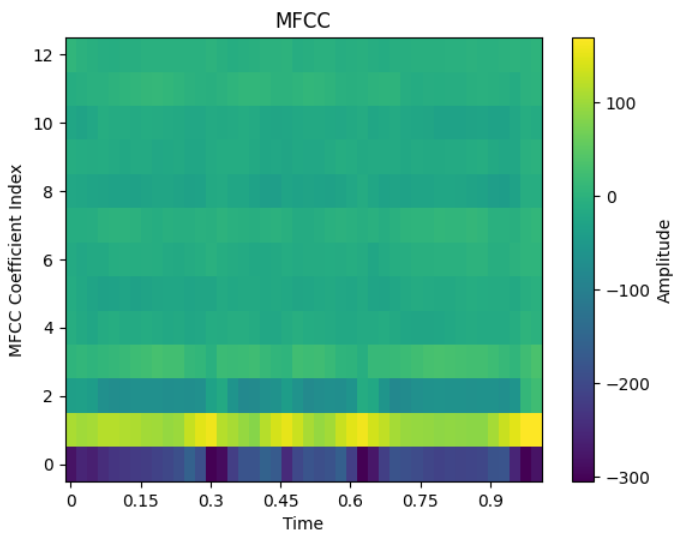
\includegraphics[width=0.8\textwidth]{kaggle_mfcc.png}
\caption{MFCC na przykładzie nagrania z bazy Kaggle}
\label{fig:kaggle_mfcc}
\end{figure}

\section{Generowanie mel-spektrogramów}
Dla drugich modeli CNN, z sekundowych segmentów wyliczono mel-spektrogramy dla 128 pasm w skali meowej. Kod tworzący mel-spektrogramy przedstawiono w Listing~\ref{lst:melspectrogram}, a jego obraz zaprezentowano na rysunku~\ref{fig:kaggle_melspectrogram}
\begin{lstlisting}[caption=Funkcja tworząca spektrogram melowy, label={lst:melspectrogram}, captionpos=b]
def create_melspectrogram(segmented_dir, n_mels=128):
    segmented_dir = Path(segmented_dir)
    X = []
    y = []
    labels = [f.name for f in segmented_dir.iterdir() if f.is_dir()]

    for label in tqdm(labels):
        for audio in (segmented_dir / label).iterdir():
            if audio.suffix == ".wav":
                signal, sr = librosa.load(audio, sr=None)
                melspectrogram = librosa.feature.melspectrogram(y=signal,   sr=sr,  n_mels=n_mels,  fmax=sr/2)
                X.append(melspectrogram)
                y.append(label)
            
    X = np.array(X)
    X = np.expand_dims(X, axis=-1)

    label_encoder = LabelEncoder()
    y = label_encoder.fit_transform(y)

    return X, np.array(y), label_encoder
\end{lstlisting}

\begin{figure}[H]
\centering
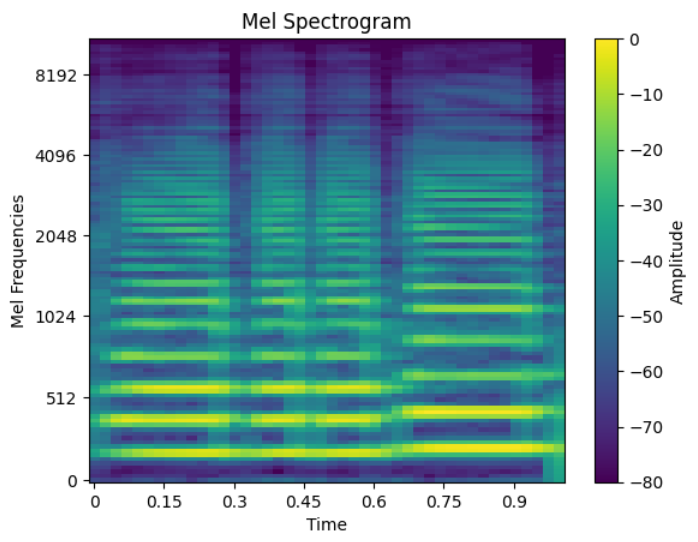
\includegraphics[width=0.8\textwidth]{kaggle_melspectrogram.png}
\caption{Mel-spektrogram na przykładzie nagrania z bazy Kaggle}
\label{fig:kaggle_melspectrogram}
\end{figure}




\chapter{Opis zastosowanych modeli klasyfikacyjnych}

\section{Przeuczenie}
Przeuczenie (Overfitting) polega na tym, że model uczy się zbyt dokładnie danych treningowych, co skutkuje niską ogólną zdolnością do generalizacji. Taki model osiąga bardzo dobre wyniki na danych treningowych, ale słabe na danych testowych. Rozwiązaniami są m.in. regularizacja, wcześniejsze zatrzymanie treningu (early stopping) i zwiększenie ilości danych~\cite{mitchell1997machine}.

\section{Modele SVM}
Do stworzenia modeli SVM ze statystykami MFCC wykorzystano klasę \texttt{SVC} z biblioteki scikit-learn~\cite{pedregosa2011scikit}. Zastosowano jądro liniowe (\texttt{kernel='linear'}), które dobrze sprawdza się w przypadku danych, które są liniowo separowalne. Model został wyuczony na zbiorze Train i oceniony na zbiorze Test. Model SVM z jądrem liniowym wybrano ze względu na jego prostotę oraz dobre właściwości generalizacji przy mniejszym ryzyku nadmiernego dopasowania (overfittingu).

\section{Modele CNN} 
Do stworzenia modeli CNN wykorzystano bibliotekę  TensorFlow~\cite{abadi2016tensorflow}. W celu sprawiedliwego porównania skuteczności obu rozwiązań, zarówno dla modeli CNN opartych na współczynnikach MFCC, jak i mel-spektrogramach, zastosowano identyczną architekturę, przedstawioną w Listing~\ref{lst:cnn_architecture}. Jako optymalizator zastosowano algorytm \texttt{Adam}, natomiast jako metrykę oceny wybrano \textit{Accuracy}~\cite{goodfellow2016deep}. Ze względu na niezbalansowany rozkład klas w zbiorze treningowym, zastosowano wagi klas obliczone przy pomocy funkcji \texttt{compute\_class\_weight} z parametrem \texttt{balanced}.

Funkcja \texttt{compute\_class\_weight} z parametrem \texttt{balanced} oblicza wagi klas na podstawie równania~\ref{eq:balanced}.

\begin{equation}
w_i = \frac{n}{k \cdot n_i}
\label{eq:balanced}
\end{equation}

gdzie:
\begin{itemize}
    \renewcommand{\labelitemi}{}
    \item \( w_i \) – waga dla klasy \( i \),
    \item \( n \) – całkowita liczba próbek w zbiorze danych,
    \item \( k \) – liczba klas,
    \item \( n_i \) – liczba próbek w klasie \( i \).
\end{itemize}

Dzięki temu klasy mniejszościowe, które mają mniej próbek, otrzymują większą wagę, co ma na celu zwiększenie ich wpływu na proces uczenia modelu.

Aby zapobiec przeuczeniu, użyto również funkcję wczesnego zatrzymania treningu \texttt{EarlyStopping} na podstawie wartości \texttt{val\_accuracy} i z parametrami: \texttt{patience=20} oraz \texttt{restore\_best\_weights=True}. Trening przeprowadzono z maksymalną liczbą 100 epok, jednak proces mógł zakończyć się wcześniej w zależności od przebiegu walidacji.

Rysunek~\ref{fig:cnn_mfcc_summary} przedstawia streszczenie modelu wygenerowane za pomocą funkcji \texttt{cnn.summary} dla modelu CNN wykorzystującego współczynniki MFCC nagrań ze zbioru IRMAS. W przypadku modeli opartych na zbiorze Kaggle zmienia się liczba parametrów w końcowej warstwie \textit{Dense} z 715 do 1040, co wynika ze zmiany liczby klas wyjściowych z 11 do 16. Dla modeli korzystających z mel-spektrogramów zmienia się również kształt danych wejściowych, a co za tym idzie, kształt danych wyjściowych warstw konwolucyjnych. 

Ostatecznie zaprezentowane modele CNN wykorzystujące zbiór Kaggle mają:
\begin{itemize} 
    \item 407 248 \textit{wszystkich parametrów};
    \item 406 288 \textit{trenowalnych parametrów};
    \item 960 \textit{nietrenowalnych parametrów}.
 \end{itemize}

Zaprezentowane modele CNN wykorzystujące zbiór IRMAS mają natomiast:
\begin{itemize} 
    \item 406 923 \textit{wszystkich parametrów};
    \item 405 963 \textit{trenowalnych parametrów};
    \item 960 \textit{nietrenowalnych parametrów}.
 \end{itemize}

\begin{lstlisting}[caption=Architektura modeli CNN, label={lst:cnn_architecture}, captionpos=b]
class_weights = compute_class_weight(class_weight='balanced', classes=np.unique(y_train), y=y_train)
class_weights_dict = dict(enumerate(class_weights))

cnn = models.Sequential([
    layers.Input(shape=(X.shape[1], X.shape[2], 1)),
    layers.Conv2D(32, (3, 3), activation='relu', padding='same'),
    layers.BatchNormalization(),
    layers.MaxPooling2D(pool_size=(2, 2), padding='same'),
    layers.Dropout(0.3),

    layers.Conv2D(64, (3, 3), activation='relu', padding='same'),
    layers.BatchNormalization(),
    layers.MaxPooling2D(pool_size=(2, 2), padding='same'),
    layers.Dropout(0.3),

    layers.Conv2D(128, (3, 3), activation='relu', padding='same'),
    layers.BatchNormalization(),
    layers.MaxPooling2D(pool_size=(2, 2), padding='same'),
    layers.Dropout(0.4),

    layers.Conv2D(256, (3, 3), activation='relu', padding='same'),
    layers.BatchNormalization(),
    layers.GlobalAveragePooling2D(),

    layers.Dense(64, activation='relu'),
    layers.Dropout(0.5),
    layers.Dense(len(np.unique(y)), activation='softmax')
])

cnn.compile(optimizer='adam',
    loss=losses.SparseCategoricalCrossentropy(),
    metrics=['accuracy'])
\end{lstlisting}

\subsection{Splot}
Splot (convolution) to podstawowa operacja wykorzystywana w sieciach neuronowych typu CNN, która polega na przetwarzaniu danych wejściowych przy użyciu filtrów (jąder konwolucyjnych). Splot jest operacją matematyczną, w której filtr przesuwa się po danych wejściowych i wykonuje operację mnożenia elementów filtru przez odpowiadające im wartości w danych wejściowych, a następnie sumuje te wyniki~\cite{goodfellow2016deep}.

Dla jednego wymiaru, operacja splotu może zostać opisana za pomocą równania~\ref{eq:convolution1}:
\begin{equation}
y(t) = (x * w)(t) = \sum_{k=0}^{K-1} x(t-k) \cdot w(k)
\label{eq:convolution1}
\end{equation}

gdzie:
\begin{itemize}
    \renewcommand{\labelitemi}{}
    \item \( x(t) \) – dane wejściowe,
    \item \( w(k) \) – filtr (jądro konwolucyjne),
    \item \( y(t) \) – wynik operacji splotu,
    \item \( K \) – długość filtru.
\end{itemize}

Dla dwóch wymiarów, jak w przypadku obrazów lub spektrogramów, splot wykonuje się na obu osiach (wysokość i szerokość) obrazu. Operację można zapisać następująco, jak w równaniu~\ref{eq:convolution2}:
\begin{equation}
y(i,j) = (x * w)(i,j) = \sum_{m=0}^{M-1} \sum_{n=0}^{N-1} x(i+m, j+n) \cdot w(m,n)
\label{eq:convolution2}
\end{equation}

gdzie:
\begin{itemize}
    \renewcommand{\labelitemi}{}
    \item \( x(i,j) \) – wartość w punkcie \((i,j)\) obrazu wejściowego,
    \item \( w(m,n) \) – wartość w punkcie \((m,n)\) filtru,
    \item \( y(i,j) \) – wynik operacji splotu w punkcie \((i,j)\),
    \item \( M \) i \( N \) – wymiary filtru.
\end{itemize}

Operacja splotu pozwala na wyodrębnienie cech, takich jak krawędzie, tekstury i wzory, co jest kluczowe w zadaniach związanych z analizą obrazów, dźwięków i innych danych przestrzennych. Dzięki wykorzystaniu filtrów, które uczą się w trakcie procesu treningowego, sieci neuronowe mogą rozpoznawać specyficzne cechy w danych, co czyni je bardzo efektywnymi w analizie różnorodnych typów danych wejściowych.

\subsection{Warstwa konwolucyjna}
Warstwa konwolucyjna \texttt{Conv2D} to podstawowy element sieci neuronowych typu CNN, który realizuje operację splotu na danych wejściowych, wykorzystując uczone podczas treningu filtry. Pozwala to na automatyczne wykrywanie istotnych cech, takich jak krawędzie, tekstury czy wzory. Zastosowanie funkcji aktywacji \texttt{ReLU} wprowadza nieliniowość, co umożliwia modelowi odwzorowanie bardziej złożonych zależności. Ustawienie parametru \texttt{padding='same'} zapewnia, że wymiary danych nie ulegają zmianie po przejściu przez warstwę. W kontekście rozpoznawania instrumentów muzycznych, warstwa ta umożliwia wyodrębnienie charakterystycznych wzorców częstotliwościowych, przy zachowaniu pełnej informacji czasowo-częstotliwościowej.

\subsection{Warstwy poolingowe}
Warstwy poolingowe \texttt{MaxPooling2D} z ustawieniem \texttt{padding='same'} zachowują wymiary danych wejściowych, co oznacza, że rozdzielczość danych nie jest zmniejszana, a liczba parametrów w dalszych warstwach sieci nie ulega redukcji w wyniku poolingowania. Pomimo braku redukcji wymiarów, pooling zwiększa efektywność obliczeniową, a także pomaga w uzyskaniu bardziej odpornych reprezentacji danych, które są mniej podatne na drobne przesunięcia lub deformacje w danych wejściowych. W przypadku rozpoznawania instrumentów muzycznych, pooling może zwiększyć odporność modelu na niewielkie zmiany w jakości dźwięku lub w jego długości.

\subsection{Normalizacja wsadowa}
Normalizacja wsadowa (\texttt{BatchNormalization}) to technika, która przyspiesza i stabilizuje proces uczenia. Polega na normalizowaniu danych w każdej warstwie sieci, aby poprawić konwergencję i zmniejszyć zależność od inicjalizacji parametrów. Zastosowanie tej metody zmniejsza również ryzyko przeuczenia modelu i sprawia, że sieć jest bardziej stabilna podczas treningu.

\subsection{Warstwa dropout}
Warstwa \texttt{Dropout} jest używana do losowego wyłączania części neuronów w trakcie treningu, co zmniejsza ryzyko overfittingu. Działanie warstwy polega na wyłączaniu neuronów z sieci na etapie treningu w sposób losowy, co zmusza sieć do nauki bardziej ogólnych cech, zamiast zapamiętywania specyficznych detali, które mogą prowadzić do przeuczenia.

\subsection{Warstwy gęsto połączone}
Na końcu sieci neuronowej znajdują się warstwy w pełni połączone (\texttt{Dense}), które są odpowiedzialne za przetwarzanie cech wyodrębnionych przez wcześniejsze warstwy. Każdy neuron w warstwie \texttt{Dense} jest połączony z wszystkimi neuronami w poprzedniej warstwie, co pozwala na efektywną klasyfikację na podstawie tych cech. Ostatnia warstwa sieci zakończona jest funkcją aktywacji \texttt{softmax}, która przekształca wyniki na prawdopodobieństwa klas, co umożliwia przypisanie próbki do jednego z instrumentów.


\begin{figure}
\centering
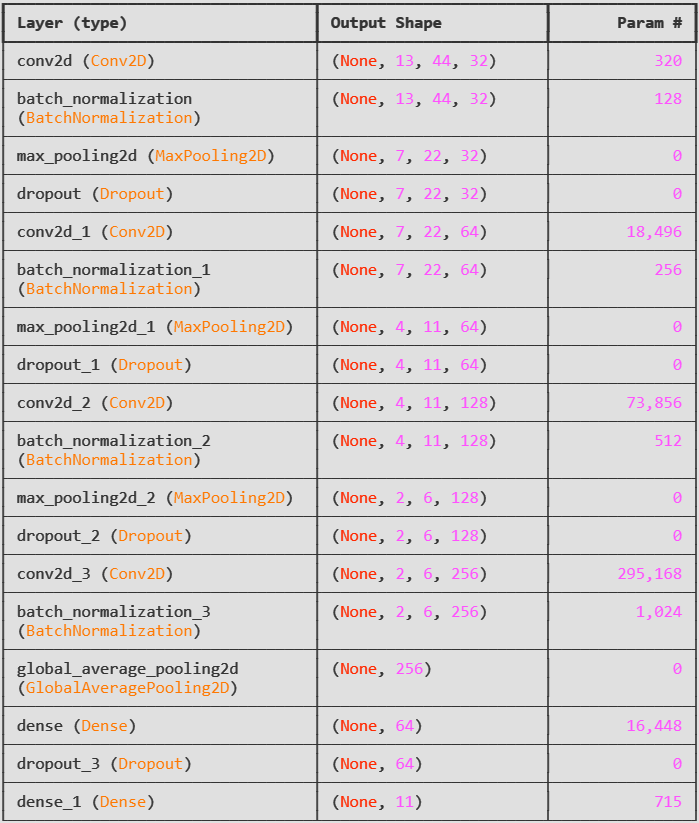
\includegraphics[width=0.8\textwidth]{cnn_mfcc_summary.png}
\caption{Wynik metody cnn.summary dla modelu CNN wykorzystującego współczynniki MFCC nagrań ze zbioru IRMAS}
\label{fig:cnn_mfcc_summary}
\end{figure}




\chapter{Wyniki i analiza eksperymentów}

\section{Kryteria oceny i metryki}
Do oceny i analizy wydajności modeli zastosowano szereg metryk. Wśród nich znalazły się: Dokładność (Accuracy), Precyzja (Precision), Czułość (Recall) oraz F1-score. Wybór tych metryk był podyktowany ich zdolnością do uchwycenia różnych rodzajów błędów oraz tendencji, które mogą negatywnie wpływać na skuteczność modeli. Ma to szczególne znaczenie w przypadku klasyfikacji z wieloma klasami i nierównowagą klas, co stanowi istotny aspekt danych używanych w niniejszej pracy.

\subsection{Dokładność}
Dokładność (\textit{Accuracy}) mierzy ogólną skuteczność modelu, czyli stosunek poprawnych przewidywań do wszystkich przewidywań. Definicję tej metryki zawiera równanie~\ref{eq:accuracy}.
\begin{equation}
\text{Accuracy} = \frac{\sum_{i=1}^n \text{TP}_i}{\sum_{i=1}^n \left( \text{TP}_i + \text{FP}_i + \text{FN}_i + \text{TN}_i \right)}
\label{eq:accuracy}
\end{equation}
gdzie:
\begin{itemize}
    \renewcommand{\labelitemi}{}
    \item \(\text{TP}_i\) – liczba prawdziwych pozytywnych dla klasy \(i\),
    \item \(\text{FP}_i\) – liczba fałszywych pozytywnych dla klasy \(i\),
    \item \(\text{FN}_i\) – liczba fałszywych negatywnych dla klasy \(i\),
    \item \(\text{TN}_i\) – liczba prawdziwych negatywnych dla klasy \(i\).
\end{itemize}

\subsection{Precyzja}
Precyzja (\textit{Precision}) dla klasy \(i\) określa, jaki procent próbek zaklasyfikowanych jako pozytywne (klasa \(i\)) rzeczywiście należy do tej klasy. Definicję tej metryki zawiera równanie~\ref{eq:precision}.
\begin{equation}
\text{Precision}_i = \frac{\text{TP}_i}{\text{TP}_i + \text{FP}_i}
\label{eq:precision}
\end{equation}
gdzie:
\begin{itemize}
    \renewcommand{\labelitemi}{}
    \item \(\text{TP}_i\) – liczba prawdziwych pozytywnych dla klasy \(i\),
    \item \(\text{FP}_i\) – liczba fałszywych pozytywnych dla klasy \(i\).
\end{itemize}

\subsection{Czułość}
Czułość (\textit{Recall}), znana również jako trafność lub True Positive Rate, dla klasy \(i\) określa, jaki procent rzeczywistych pozytywnych przypadków dla klasy \(i\) został poprawnie wykryty. Definicję tej metryki zawiera równanie~\ref{eq:recall}.
\begin{equation}
\text{Recall}_i = \frac{\text{TP}_i}{\text{TP}_i + \text{FN}_i}
\label{eq:recall}
\end{equation}
gdzie:
\begin{itemize}
    \renewcommand{\labelitemi}{}
    \item \(\text{TP}_i\) – liczba prawdziwych pozytywnych dla klasy \(i\),
    \item \(\text{FN}_i\) – liczba fałszywych negatywnych dla klasy \(i\).
\end{itemize}

\subsection{F1-score}
F1-score (\textit{F1-score}) to harmoniczna średnia precyzji i czułości dla klasy \(i\). Używana jest, gdy chcemy zrównoważyć obie te metryki. Definicję tej metryki zawiera równanie~\ref{eq:f1}.
\begin{equation}
F_1 = 2 \cdot \frac{\text{Precision}_i \cdot \text{Recall}_i}{\text{Precision}_i + \text{Recall}_i}
\label{eq:f1}
\end{equation}
gdzie:
\begin{itemize}
    \renewcommand{\labelitemi}{}
    \item \(\text{Precision}_i\) – precyzja dla klasy \(i\),
    \item \(\text{Recall}_i\) – czułość dla klasy \(i\).
\end{itemize}

\subsection{Średnia makro}
Średnia makro (\textit{Macro average}) oblicza średnią metryki (np. Precyzji, Czułości, F1-score) dla każdej klasy z osobna, traktując wszystkie klasy równoważnie, niezależnie od ich rozkładu. Jest to przydatne w przypadku nierównowagi klas, ponieważ nie faworyzuje klas o większej liczbie próbek.

\subsection{Średnia ważona}
Średnia ważona (\textit{Weighted average}) oblicza średnią metryki z uwzględnieniem liczebności każdej klasy. Jest to przydatne, gdy chcemy, aby klasy bardziej reprezentowane miały większy wpływ na wynik końcowy metryki.

\section{Porównanie wyników między modelami}
W kolejnych tabelach zaprezentowano \textit{Classification Report}, pokazujący wyniki osiągnięte przez dany model na zbiorze \textit{Test}. We wszystkich przypadkach metryki \textit{Precision}, \textit{Recall} oraz \textit{F1-score} nie odbiegały znacząco od \textit{Accuracy} i były podobne zarówno dla \textit{Macro Average} jak i \textit{Weighted Average}. Świadczy to o tym, że wartości \textit{Accuracy} precyzyjnie określają dokładność modeli i nie ukrywają innych niedociągnięć. W związku z tym, w dalszej części analizy wartość \textit{Accuracy} będzie traktowana jako domyślna miara sukcesu modelu w klasyfikacji instrumentów.

\subsection{Modele SVM wykorzystujące statystyki MFCC}
Wyniki klasyfikacji dla modeli SVM zostały przedstawione w tabelach~\ref{tab:svm_mfcc_kaggle} i~\ref{tab:svm_mfcc_IRMAS}. Modele te wykazały różnorodne wyniki w zależności od klasy instrumentu. \textit{Accuracy} w przypadku bazy Kaggle wynosi 0,78. Warto zauważyć, że dla niektórych klas, takich jak Cowbell (\textit{Precision} 0,95, \textit{Recall} 0,95, \textit{F1-Score} 0,95), model osiągnął doskonałe wyniki. Natomiast inne klasy, takie jak Clarinet (\textit{Precision} 0.58, \textit{Recall} 0,54, \textit{F1-Score} 0,56), uzyskały niższe wartości, co sugeruje problemy z dokładnym rozróżnieniem bardziej skomplikowanych instrumentów przy użyciu jedynie statystyk MFCC. Dla bazy IRMAS \textit{Accuracy} modelu wynosi 0,48, co wskazuje na niższą skuteczność na tym zbiorze danych w porównaniu do bazy Kaggle.

\begin{table}[H]
\centering
\caption{Raport klasyfikacji modelu SVM wykorzystującego statystyki MFCC dla bazy danych Kaggle}
\label{tab:svm_mfcc_kaggle}
\begin{tabular}{lcccc}
\toprule
\textbf{Klasa} & \textbf{Precyzja} & \textbf{Czułość} & \textbf{F1-Score} & \textbf{Wsparcie} \\
\midrule
gitara akustyczna (Acoustic guitar) & 0,57 & 0,76 & 0,65 & 21 \\
bęben basowy (Bass drum) & 0,92 & 0,85 & 0,88 & 13 \\
wiolonczela (Cello) & 0,87 & 0,80 & 0,83 & 25 \\
klarnet (Clarinet) & 0,58 & 0,54 & 0,56 & 26 \\
krowi dzwonek (Cowbell) & 0,95 & 0,95 & 0,95 & 19 \\
kontrabas (Double bass) & 0,86 & 1,00 & 0,92 & 18 \\
fortepian elektryczny (Electric piano) & 0,77 & 0,67 & 0,71 & 15 \\
flet (Flute) & 0,57 & 0,65 & 0,61 & 26 \\
dzwonki (Glockenspiel) & 0,88 & 1,00 & 0,93 & 14 \\
harmonijka ustna (Harmonica) & 0,88 & 0,78 & 0,82 & 18 \\
hi-hat (Hi-hat) & 0,82 & 1,00 & 0,90 & 18 \\
obój (Oboe) & 0,65 & 0,85 & 0,74 & 20 \\
saksofon (Saxophone) & 0,80 & 0,71 & 0,75 & 51 \\
tamburyn (Tambourine) & 0,95 & 0,95 & 0,95 & 19 \\
trąbka (Trumpet) & 0,88 & 0,82 & 0,85 & 17 \\
skrzypce (Violin or fiddle) & 0,88 & 0,70 & 0,78 & 50 \\
\midrule
\textbf{Dokładność} & & & \textbf{0,78} & 370 \\
\textbf{Średnia makro} & 0,80 & 0,81 & 0,80 & 370 \\
\textbf{Średnia ważona} & 0,79 & 0,78 & 0,78 & 370 \\
\bottomrule
\end{tabular}
\end{table}

\begin{table}[H]
\centering
\caption{Raport klasyfikacji modelu SVM wykorzystującego statystyki MFCC dla bazy danych IRMAS}
\label{tab:svm_mfcc_IRMAS}
\begin{tabular}{lcccc}
\toprule
\textbf{Klasa} & \textbf{Precyzja} & \textbf{Czułość} & \textbf{F1-Score} & \textbf{Wsparcie} \\
\midrule
wiolonczela (cel) & 0,51 & 0,62 & 0,56 & 78 \\
klarnet (cla) & 0,54 & 0,42 & 0,47 & 101 \\
flet (flu) & 0,45 & 0,33 & 0,38 & 90 \\
gitara akustyczna (gac) & 0,45 & 0,49 & 0,47 & 127 \\
gitara elektryczna (gel) & 0,35 & 0,49 & 0,41 & 152 \\
organy (org) & 0,44 & 0,59 & 0,50 & 136 \\
fortepian (pia) & 0,53 & 0,55 & 0,54 & 144 \\
saksofon (sax) & 0,36 & 0,24 & 0,29 & 125 \\
trąbka (tru) & 0,52 & 0,41 & 0,46 & 116 \\
skrzypce (vio) & 0,63 & 0,44 & 0,52 & 116 \\
głos ludzki (voi) & 0,60 & 0,65 & 0,63 & 156 \\
\midrule
\textbf{Dokładność} & & & \textbf{0,48} & 1341 \\
\textbf{Średnia makro} & 0,49 & 0,47 & 0,47 & 1341 \\
\textbf{Średnia ważona} & 0,49 & 0,48 & 0,48 & 1341 \\
\bottomrule
\end{tabular}
\end{table}

\subsection{Modele CNN wykorzystujące współczynniki MFCC}
Na rysunkach~\ref{fig:kaggle_cnn_mfcc_training_curves} i~\ref{fig:IRMAS_cnn_mfcc_training_curves} przedstawiono wykresy zmian wartości \textit{Accuracy} i \textit{Loss} modeli CNN wykorzystujących współczynniki MFCC dla kolejnych epok. W przypadku bazy Kaggle, \textit{Accuracy} stabilnie rośnie zarówno dla \textit{Train} jak i \textit{Validation}, co wskazuje na brak overfittingu. \textit{Validation} ma wyższe wartości niż \textit{Train} i przekrocza \textit{Accuracy} 0,9, co świadczy o wyjątkowo trafnym rozpoznawaniu cech poszczególnych instrumentów. Dla bazy IRMAS model początkowo usprawnia wykrywanie cech, co widać w stabilnym wzroście \textit{Accuracy} dla zrówno \textit{Train}, jak i \textit{Validation}, jednak koło 50 epoki zaczyna się overfitting, co widać w dysproporcji wzrostu \textit{Train} do \textit{Validation}. Na podstawie wyników przedstawionych w tabelach~\ref{tab:cnn_mfcc_kaggle} oraz~\ref{tab:cnn_mfcc_IRMAS} widać, że wynik dokładności dla Kaggle wyniósł 0,92, co stanowi wzrost o 0,24 w stosunku do modelu SVM, natomiast w przypadku IRMAS wyniósł 0,69, czyli o 0,21 więcej od modelu SVM.

\begin{figure}[H]
\centering
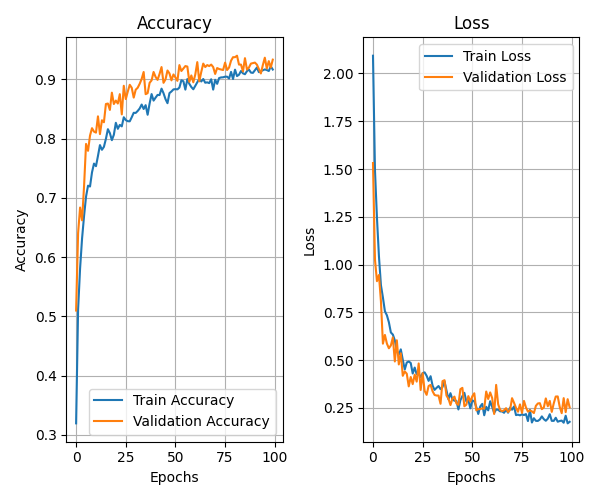
\includegraphics[width=0.8\textwidth]{kaggle_cnn_mfcc_training_curves.png}
\caption{Wykresy zmian wartości Accuracy i Loss modelu CNN wykorzystującego współczynniki MFCC dla bazy Kaggle}
\label{fig:kaggle_cnn_mfcc_training_curves}
\end{figure}

\begin{figure}[H]
\centering
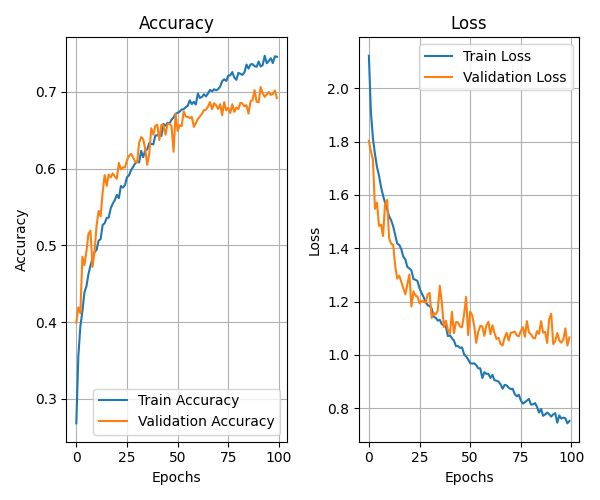
\includegraphics[width=0.8\textwidth]{IRMAS_cnn_mfcc_training_curves.png}
\caption{Wykresy zmian wartości Accuracy i Loss modelu CNN wykorzystującego współczynniki MFCC dla bazy IRMAS}
\label{fig:IRMAS_cnn_mfcc_training_curves}
\end{figure}

\begin{table}[H]
\centering
\caption{Raport klasyfikacji modelu CNN wykorzystującego współczynniki MFCC dla bazy Kaggle}
\label{tab:cnn_mfcc_kaggle}
\begin{tabular}{lcccc}
\toprule
\textbf{Klasa} & \textbf{Precyzja} & \textbf{Czułość} & \textbf{F1-Score} & \textbf{Wsparcie} \\
\midrule
gitara akustyczna (Acoustic guitar) & 0,97 & 0,91 & 0,94 & 98 \\
bęben basowy (Bass drum) & 0,82 & 0,93 & 0,88 & 15 \\
wiolonczela (Cello) & 0,95 & 0,90 & 0,93 & 21 \\
klarnet (Clarinet) & 0,84 & 0,86 & 0,85 & 37 \\
krowi dzwonek (Cowbell) & 0,78 & 0,98 & 0,87 & 63 \\
kontrabas (Double bass) & 0,96 & 0,95 & 0,95 & 91 \\
fortepian elektryczny (Electric piano) & 0,94 & 0,91 & 0,92 & 322 \\
flet (Flute) & 0,95 & 0,94 & 0,95 & 167 \\
dzwonki (Glockenspiel) & 0,90 & 0,93 & 0,91 & 151 \\
harmonijka ustna (Harmonica) & 1,00 & 0,93 & 0,96 & 28 \\
hi-hat (Hi-hat) & 0,85 & 0,85 & 0,85 & 71 \\
obój (Oboe) & 0,95 & 0,84 & 0,89 & 95 \\
saksofon (Saxophone) & 0,76 & 1,00 & 0,86 & 16 \\
tamburyn (Tambourine) & 1,00 & 0,96 & 0,98 & 23 \\
trąbka (Trumpet) & 0,95 & 0,94 & 0,95 & 107 \\
skrzypce (Violin or fiddle) & 0,94 & 0,95 & 0,95 & 197 \\
\midrule
\textbf{Dokładność} & & & \textbf{0,92} & 1502 \\
\textbf{Średnia makro} & 0,91 & 0,92 & 0,91 & 1502 \\
\textbf{Średnia ważona} & 0,93 & 0,92 & 0,92 & 1502 \\
\bottomrule
\end{tabular}
\end{table}

\begin{table}[H]
\centering
\caption{Raport klasyfikacji modelu CNN wykorzystującego współczynniki MFCC dla bazy IRMAS}
\label{tab:cnn_mfcc_IRMAS}
\begin{tabular}{lcccc}
\toprule
\textbf{Klasa)} & \textbf{Precyzja} & \textbf{Czułość} & \textbf{F1-Score} & \textbf{Wsparcie} \\
\midrule
wiolonczela (cel) & 0,63 & 0,86 & 0,73 & 233 \\
klarnet (cla) & 0,64 & 0,63 & 0,63 & 303 \\
flet (flu) & 0,53 & 0,59 & 0,56 & 270 \\
gitara akustyczna (gac) & 0,66 & 0,85 & 0,74 & 382 \\
gitara elektryczna (gel) & 0,70 & 0,67 & 0,68 & 456 \\
organy (org) & 0,76 & 0,73 & 0,74 & 409 \\
fortepian (pia) & 0,73 & 0,64 & 0,68 & 433 \\
saksofon (sax) & 0,67 & 0,51 & 0,58 & 376 \\
trąbka (tru) & 0,76 & 0,68 & 0,72 & 346 \\
skrzypce (vio) & 0,61 & 0,68 & 0,64 & 348 \\
głos ludzki (voi) & 0,82 & 0,74 & 0,78 & 467 \\
\midrule
\textbf{Dokładność} & & & \textbf{0,69} & 4023 \\
\textbf{Średnia makro} & 0,68 & 0,69 & 0,68 & 4023 \\
\textbf{Średnia ważona} & 0,69 & 0,69 & 0,69 & 4023 \\
\bottomrule
\end{tabular}
\end{table}

\subsection{Modele CNN wykorzystujące mel-spektrogramamy}
Modele CNN wykorzystujące mel-spektrogramamy (jak przedstawiono na rysunkach~\ref{fig:kaggle_cnn_melspectrogram_training_curves} oraz~\ref{fig:IRMAS_cnn_melspectrogram_training_curves}) charakteryzują się dużą niestabilnością dokładności \textit{Validation}, pomimo stałego wzrost maksymalnych wartości. W przypadku bazy IRMAS, gdzie jest to jeszcze bardziej utrudnione przez abstrakcyjny koncept dominującego instrumentu, występuje overfitting. Pomimo wachań, modele te osiągnęły najlepsze wyniki wśród wszystkich testowanych podejść, co widać w tabelach~\ref{tab:cnn_melspectrogram_kaggle} i~\ref{tab:cnn_melspectrogram_IRMAS}. W przypadku bazy danych Kaggle, model osiągnął dokładność taką samą jak w poprzednim modelu, czyli 0,92. W przypadku bazy danych IRMAS, wyniki dokładności wyniósł 0,75, czyli wzrósł o 0,06 w porównaniu do rozwiązania CNN ze współczynnikami MFCC.

\begin{figure}[H]
\centering
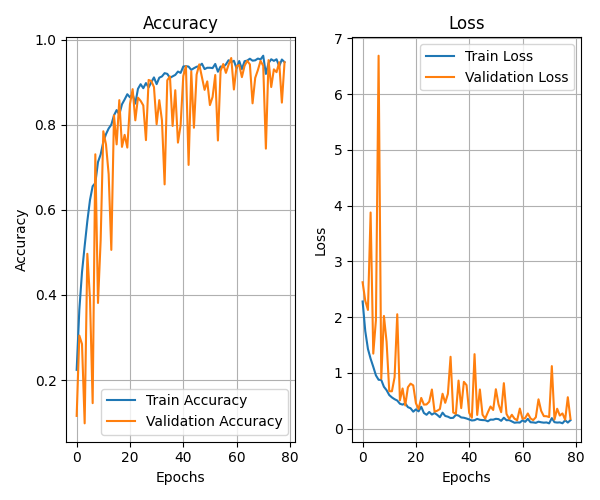
\includegraphics[width=0.8\textwidth]{kaggle_cnn_melspectrogram_training_curves.png}
\caption{Wykresy zmian wartości Accuracy i Loss modelu CNN wykorzystującego mel-spektrogramamy dla bazy danych Kaggle}
\label{fig:kaggle_cnn_melspectrogram_training_curves}
\end{figure}

\begin{figure}[H]
\centering
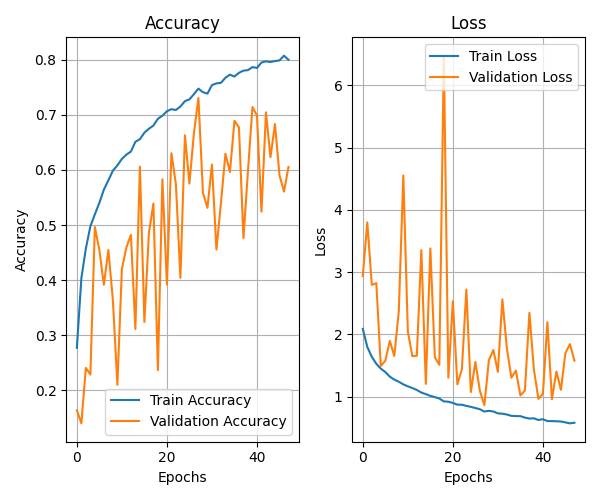
\includegraphics[width=0.8\textwidth]{IRMAS_cnn_melspectrogram_training_curves.png}
\caption{Wykresy zmian wartości Accuracy i Loss modelu CNN wykorzystującego mel-spektrogramamy dla bazy danych IRMAS}
\label{fig:IRMAS_cnn_melspectrogram_training_curves}
\end{figure}

\begin{table}[H]
\centering
\caption{Raport klasyfikacji modelu CNN wykorzystującego mel-spektrogramy dla bazy danych Kaggle}
\label{tab:cnn_melspectrogram_kaggle}
\begin{tabular}{lcccc}
\toprule
\textbf{Klasa} & \textbf{Precyzja} & \textbf{Czułość} & \textbf{F1-Score} & \textbf{Wsparcie} \\
\midrule
gitara akustyczna (Acoustic guitar) & 0,97 & 0,90 & 0,93 & 98 \\
bęben basowy (Bass drum) & 0,75 & 1,00 & 0,86 & 15 \\
wiolonczela (Cello) & 0,87 & 0,95 & 0,91 & 21 \\
klarnet (Clarinet) & 0,77 & 0,89 & 0,82 & 37 \\
krowi dzwonek (Cowbell) & 0,83 & 0,95 & 0,89 & 63 \\
kontrabas (Double bass) & 0,96 & 0,99 & 0,97 & 91 \\
fortepian elektryczny (Electric piano) & 0,99 & 0,86 & 0,92 & 322 \\
flet (Flute) & 0,88 & 0,99 & 0,93 & 167 \\
dzwonki (Glockenspiel) & 0,94 & 0,93 & 0,94 & 151 \\
harmonijka ustna (Harmonica) & 1,00 & 0,93 & 0,96 & 28 \\
hi-hat (Hi-hat) & 0,86 & 0,94 & 0,90 & 71 \\
obój (Oboe) & 0,99 & 0,88 & 0,93 & 95 \\
saksofon (Saxophone) & 0,75 & 0,94 & 0,83 & 16 \\
tamburyn (Tambourine) & 0,92 & 1,00 & 0,96 & 23 \\
trąbka (Trumpet) & 0,83 & 0,94 & 0,88 & 107 \\
skrzypce (Violin or fiddle) & 0,97 & 0,92 & 0,95 & 197 \\
\midrule
\textbf{Dokładność} & & & \textbf{0,92} & 1502 \\
\textbf{Średnia makro} & 0,89 & 0,94 & 0,91 & 1502 \\
\textbf{Średnia ważona} & 0,93 & 0,92 & 0,92 & 1502 \\
\bottomrule
\end{tabular}
\end{table}

\begin{table}[H]
\centering
\caption{Raport klasyfikacji modelu CNN wykorzystującego mel-spektrogramy dla bazy danych IRMAS}
\label{tab:cnn_melspectrogram_IRMAS}
\begin{tabular}{lcccc}
\toprule
\textbf{Klasa} & \textbf{Precyzja} & \textbf{Czułość} & \textbf{F1-Score} & \textbf{Wsparcie} \\
\midrule
wiolonczela (cel) & 0,62 & 0,88 & 0,73 & 233 \\
klarnet (cla) & 0,79 & 0,69 & 0,74 & 303 \\
flet (flu) & 0,78 & 0,68 & 0,72 & 270 \\
gitara akustyczna (gac) & 0,84 & 0,71 & 0,77 & 382 \\
gitara elektryczna (gel) & 0,75 & 0,61 & 0,67 & 456 \\
organy (org) & 0,94 & 0,79 & 0,86 & 409 \\
fortepian (pia) & 0,72 & 0,88 & 0,79 & 433 \\
saksofon (sax) & 0,78 & 0,50 & 0,61 & 376 \\
trąbka (tru) & 0,77 & 0,82 & 0,79 & 346 \\
skrzypce (vio) & 0,51 & 0,77 & 0,62 & 348 \\
głos ludzki (voi) & 0,85 & 0,89 & 0,87 & 467 \\
\midrule
\textbf{Dokładność} & & & \textbf{0,75} & 4023 \\
\textbf{Średnia makro} & 0,76 & 0,75 & 0,74 & 4023 \\
\textbf{Średnia ważona} & 0,77 & 0,75 & 0,75 & 4023 \\
\bottomrule
\end{tabular}
\end{table}

\section{Analiza wyników}
Ostateczne porównanie dokładności wszystkich modeli dla obu baz danych przedstawiono w tabeli~\ref{tab:comparison_accuracy_models}. Można zauważyć, że we wszystkich przypadkach zbiór Kaggle osiągnął lepsze wyniki niż zbiór IRMAS. Wynika to z faktu, że w zbiorze IRMAS obecność instrumentów tła znacząco utrudnia generalizację modelu. Ma to szczególne znaczenie w przypadku wykorzystania cech MFCC, ponieważ trudniej jest w nich wyodrębnić dominujący instrument. Zjawisko to widoczne jest w tym, że zastosowanie mel-spektrogramów skutkuje wzrostem dokładności modeli trenowanych na zbiorze IRMAS, podczas gdy w przypadku zbioru Kaggle takiego wzrostu nie zaobserwowano. Może to świadczyć o tym, że model był w stanie wydobyć nowe cechy poprawiające jego zdolność do generalizacji. Najsłabiej wypadły modele SVM. Pokazuje to, że współczynniki MFCC, a nie jedynie ich statystyki, umożliwiają modelom CNN uchwycenie zależności przestrzennych między różnymi punktami w czasie, co przekłada się na lepszą skuteczność klasyfikacji w porównaniu do standardowego podejścia SVM.

\begin{table}[H]
\centering
\caption{Porównanie Accuracy modeli SVM wykorzystujących statystyki MFCC, CNN wykorzystujących współczynniki MFCC oraz CNN wykorzystujących mel-spektrogramamy dla zbiorów danych Kaggle i IRMAS}
\label{tab:comparison_accuracy_models}
\begin{tabular}{lccc}
\toprule
\textbf{} & \text{SVM (statystyki MFCC)} & \text{CNN (MFCC)} & \text{CNN (Mel-spektrogram)} \\
\midrule
Kaggle & 0,78 & 0,92 & 0,92 \\
IRMAS & 0,48 & 0,69 & 0,75 \\
\bottomrule
\end{tabular}
\end{table}

\section{Sugestie ulepszeń i kierunki dalszych badań}
Najbardziej obiecującym modelem okazała się konwolucyjna sieć neuronowa (CNN) wykorzystująca mel-spektrogramy. Model ten wykazuje wysoką zdolność do generalizacji nagrań o zróżnicowanej jakości oraz z obecnością innych instrumentów w tle. W celu dalszego zwiększenia dokładności klasyfikacji na tego typu danych, model powinien zostać rozszerzony o dodatkowe warstwy ukryte. Umożliwiłoby to lepsze uchwycenie bardziej abstrakcyjnych cech, jaką jest dominujący instrument w nagraniu. Dodatkowo, zwiększenie liczby oraz różnorodności danych treningowych mogłoby opóźnić moment wystąpienia zjawiska overfittingu, co w konsekwencji przyczyniłoby się do dalszej poprawy ogólnej skuteczności modelu.




\chapter{Podsumowanie}
Celem niniejszej pracy dyplomowej było porównanie skuteczności klasycznych i głębokich metod uczenia maszynowego w zadaniu rozpoznawania instrumentów muzycznych na podstawie cech dźwiękowych. W tym celu wykorzystano klasyfikator maszyn wektorów nośnych (SVM), zrealizowany przy użyciu biblioteki scikit-learn oraz konwolucyjną sieć neuronową (CNN) zaimplementowaną z wykorzystaniem biblioteki TensorFlow. Modele SVM wykorzystywały jedynie statystyki MFCC, natomiast CNN zostały przetestowane w dwóch wersjach: wykorzystując współczynniki MFCC oraz wykorzystując mel-spektrogramy. Eksperymenty przeprowadzono na dwóch zbiorach danych: IRMAS, zawierającym próbki dźwiękowe oznaczone jednym z 11 dominujących instrumentów, oraz Kaggle, zawierającym nagrania jednego z 16 instrumentów. Wyniki uzyskane w eksperymentach wykazały, że dla zbioru Kaggle modele CNN (wykorzystujące współczynniki MFCC i mel-spektrogramy) osiągnęły lepsze wyniki w porównaniu do modelu SVM, który wykazał się dobrą wydajnością, ale przy niższej skuteczności. Z kolei dla zbioru IRMAS, modele CNN wykorzystujące mel-spektrogramamy okazały się najlepsze, oferując wyższą dokładność w porównaniu do innych podejść. Analiza wyników pokazała, że dobór odpowiednich cech oraz architektury modelu ma istotny wpływ na jakość klasyfikacji. Głębokie sieci neuronowe, mimo większych wymagań obliczeniowych, oferują lepszą zdolność do automatycznego wydobywania i analizowania złożonych wzorców w danych dźwiękowych, co czyni je preferowanym wyborem w zadaniach tego typu. Reprezentacja mel-spektrogramowa okazała się szczególnie skuteczna w przypadku bardziej złożonych zbiorów danych, jakim jest IRMAS.




\begin{thebibliography}{9}
\bibitem{mitchell1997machine}
Tom Mitchell, McGraw Hill, \textit{Machine Learning} \url{https://www.cs.cmu.edu/~tom/mlbook.html} (dostęp: 5.03.2025)

\bibitem{moguerza2006support}
Javier M. Moguerza, Alberto Muñoz, \textit{Support Vector Machines with Applications} \url{https://arxiv.org/abs/math/0612817} (dostęp: 5.03.2025)

\bibitem{goodfellow2016deep} 
Ian Goodfellow, Yoshua Bengio, Aaron Courville, \textit{Deep Learning} \url{https://www.deeplearningbook.org} (dostęp: 6.03.2025)

\bibitem{smith1997scientist} 
Steven W. Smith, \textit{The scientist and engineer's guide to digital signal processing} \url{https://www.dspguide.com/ch9.htm} (dostęp: 29.04.2025)

\bibitem{bracewell2000fourier} 
Ronald N. Bracewell, \textit{The Fourier transform and its applications} \url{https://archive.org/details/TheFourierTransformAndItsApplicationsBracewell} (dostęp: 30.04.2025)

\bibitem{gescheider2013psychophysics} 
George A. Gescheider, \textit{Psychophysics: the fundamentals} \url{https://www.taylorfrancis.com/books/mono/10.4324/9780203774458/psychophysics-george-gescheider} (dostęp: 30.04.2025)

\bibitem{jadhav2015classification} 
Priyanka S. Jadhav, \textit{Classification of musical instruments sounds by using MFCC and timbral audio descriptors} \url{https://core.ac.uk/download/pdf/539909195.pdf} (dostęp: 7.03.2025)

\bibitem{thornton2019audio}
Boyang Zhang, Jared Leitner, Sam Thornton, \textit{Audio recognition using mel spectrograms and convolution neural networks} \url{https://noiselab.ucsd.edu/ECE228_2019/Reports/Report38.pdf} (dostęp: 11.03.2025)

\bibitem{eronen2001automatic}
Antti Eronen, \textit{Automatic musical instrument recognition} \url{http://hans.fugal.net/comps/papers/eronen_2001.pdf} (dostęp: 14.1.2024)

\bibitem{herrera2003automatic}
Perfecto Herrera-Boyer, Geoffroy Peeters, Shlomo Dubnov, \textit{Automatic classification of musical instrument sounds} \url{https://www.music.mcgill.ca/~ich/classes/mumt621_14/classifiers/Herrera_timbre.pdf} (dostęp: 11.03.2025)

\bibitem{wieczorkowska2003rough}
Alicja A. Wieczorkowska, Andrzej Czyżewski \textit{Rough Set Based Automatic Classification of Musical Instrument Sounds.} \url{https://www.sciencedirect.com/science/article/pii/S1571066104807278} (dostęp: 30.04.2025)

\bibitem{wieczorkowska2008identification}
Alicja Wieczorkowska, Elżbieta Kolczyńska, \textit{Identification of Dominating Instrument in Mixes of Sounds of the Same Pitch.} \url{https://webpages.charlotte.edu/ras/mir/Paper-20.pdf} (dostęp: 30.04.2025)

\bibitem{jiang2009music}
Wenxin Jiang, Alicja Wieczorkowska, Zbigniew W. Raś, \textit{Music Instrument Estimation in Polyphonic Sound Based on Short-Term Spectrum Match.} \url{https://webpages.charlotte.edu/ras/Papers/Jiang-Ala.pdf} (dostęp: 30.04.2025)

\bibitem{bosch2012comparison}
Juan J. Bosch, Jordi Janer, Ferdinand Fuhrmann, Perfecto Herrera, \textit{A Comparison of Sound Segregation Techniques for Predominant Instrument Recognition in Musical Audio Signals.} \url{https://repositori-api.upf.edu/api/core/bitstreams/1a9d8270-b39a-415c-bf8e-984a9336f0e9/content} (dostęp: 12.02.2025)

\bibitem{kubera2013time}
Elżbieta Kubera, Alicja A. Wieczorkowska, Zbigniew W. Raś, \textit{Time Variability-Based Hierarchic Recognition of Multiple Musical Instruments in Recordings.} Chapter 15, \url{https://webpages.charlotte.edu/ras/Papers/chapter-K-W.pdf} (dostęp: 30.04.2025)

\bibitem{kursa2014multi}
Miron B. Kursa, Alicja A. Wieczorkowska, \textit{Multi-label Ferns for Efficient Recognition of Musical Instruments in Recordings.} \url{https://arxiv.org/pdf/1403.7746} (dostęp: 30.04.2025)

\bibitem{solanki2022music}
Arun Solanki, Sachin Pandey \textit{Music instrument recognition using deep convolutional neural networks} International Journal of Information Technology 14.3 (2022): 1659-1668

\bibitem{howard2018freesound}
Addison Howard, Eduardo Fonseca, Frederic Font, inversion, and Manoj Plakal,  \textit{Freesound General-Purpose Audio Tagging Challenge} \url{https://kaggle.com/competitions/freesound-audio-tagging} (dostęp: 12.02.2025)

\bibitem{bosch2012irmas}
Juan J. Bosch, Ferdinand Fuhrmann, Perfecto Herrera, \textit{IRMAS: a dataset for instrument recognition in musical audio signals} \url{https://www.upf.edu/web/mtg/irmas} (dostęp: 12.02.2025)

\bibitem{mcfee2015librosa}
McFee, Brian and Raffel, Colin and Liang, Dawen and Ellis, Daniel PW and McVicar, Matt and Battenberg, Eric and Nieto, Oriol, \textit{librosa: Audio and music signal analysis in python.} SciPy 2015 (2015): 18-24.

\bibitem{harris2020array}
Harris, Charles R and Millman, K Jarrod and Van Der Walt, St{\'e}fan J and Gommers, Ralf and Virtanen, Pauli and Cournapeau, David and Wieser, Eric and Taylor, Julian and Berg, Sebastian and Smith, Nathaniel J and others, \textit{Array programming with NumPy.} \url{https://www.nature.com/articles/s41586-020-2649-2.pdf} (dostęp: 14.03.2025)

\bibitem{mckinney2010data}
McKinney, Wes and others, \textit{Data structures for statistical computing in Python.} \url{https://pdfs.semanticscholar.org/ef4e/f7f38bb907e5d7b4df3e6ff1db269d4970f5.pdf} (dostęp: 14.03.2025)

\bibitem{pedregosa2011scikit}
Pedregosa, Fabian and Varoquaux, Ga{\"e}l and Gramfort, Alexandre and Michel, Vincent and Thirion, Bertrand and Grisel, Olivier and Blondel, Mathieu and Prettenhofer, Peter and Weiss, Ron and Dubourg, Vincent and others, \textit{Scikit-learn: Machine learning in Python} \url{https://www.jmlr.org/papers/volume12/pedregosa11a/pedregosa11a.pdf?source=post_page} (dostęp: 14.03.2025)

\bibitem{abadi2016tensorflow}
Abadi, Mart{\'\i}n and Barham, Paul and Chen, Jianmin and Chen, Zhifeng and Davis, Andy and Dean, Jeffrey and Devin, Matthieu and Ghemawat, Sanjay and Irving, Geoffrey and Isard, Michael and others, \textit{$\{$TensorFlow$\}$: a system for $\{$Large-Scale$\}$ machine learning} \url{https://www.usenix.org/system/files/conference/osdi16/osdi16-abadi.pdf} (dostęp: 14.03.2025)
\end{thebibliography}

\beforelastpage

\end{document}
